\section{Segmentacja tablic rejestracyjnych}
Podczas pracy nad algorytmami segmentacji obrazu, przede wszystkim skupiłem się na problemie segmentacji tablic rejestracyjnych. Segmentacja jest kluczowym elementem procesu identyfikacji tablicy rejestracyjnej.\\
Algorytmy rozpoznawania tablic rejestracyjnych wykorzystywane są bardzo często w rozwiązaniach przemysłowych, przez co wymagana jest wysoka jakość zwracanych wyników.\\
Ze względu na różnorodność formatów tablic rejestracyjnych, jakie mogą wystąpić, oraz dodatkowych utrudnień związanych z niedoskonałością środowiska w którym wykonywany jest obraz, problem segmentacji tablic rejestracyjnych nie jest problemem łatwym do rozwiązania.
\paragraph{}
Obrazy tablic rejestracyjnych, ze względu na warunki w jakich są wykonywane, nie zawierają jedynie tekstu, który jest łatwy do analizy. Obrazy często zawierają artefakty, tablice mogą być zanieczyszczone, lub ze względu na warunki atmosferyczne, obraz może być niejednolicie oświetlony. Opisałem problemy, z jakimi spotkałem się, analizując zestaw danych testowych, wraz z proponowanymi przeze mnie możliwościami rozwiązania problemów.\\
W tym rozdziale będę stosował wykorzystywał formę zapisu wzorów matematycznych stosowaną w języku programowania C++.
\subsection{Różne kolory tablic rejestracyjnych}\label{ssec:different_backgrounds}
Algorytmy segmentacji tablic rejestracyjnych które zaprezentuję w dalszej części pracy, wymagają, aby tło tablic rejestracyjnych było jaśniejsze od tekstu. Dlatego opracowałem algorytm, który wykrywa odwrotną sytuację, i w razie potrzeby, odwróci kolory obrazu.\\
Pierwszym pomysłem było zastosowanie lokalnego progowania, a następnie policzenie czarnych oraz białych pikseli, i w zależności od tego, który kolor występuje częściej, określić tło tablicy rejestracyjnej. Metoda ta okazała się w większości przypadków skuteczna. Algorytm nie zwracał jednak poprawnych rezultatów w przypadku, gdy tablica rejestracyjna wykonana była pod kątem, i nie można było wykadrować obrazu w taki sposób, aby pozbyć się nieporządanych pikseli. Rysunek~\ref{fig:detect_bg_bad} przedstawia ten problem. Tablica rejestracyjna zajmuje większą część obrazu, jednak pomimo tego, została sklasyfikowana przez algorytm jako tablica z czarnym tłem. Wynika to z faktu, iż na tablicy pozostały znaki, które również zajmują znaczącą powierzchnię obrazu. Następnie spróbowałem zastosować operację zamknięcia regionu, która poprawnie usunęła znaki z obrazu. Nie zadziałała jednak w przypadku białych znaków na czarnym tle. \\
Zamiast operacji morfologicznej, zastosowałem rozmycie medianowe, które dało poprawny efekt zarówno dla czarnych znaków na białym tle, jak również dla białych znaków na czarnym tle. Na rysunku~\ref{fig:detect_bg_ok} przedstawiony został wynik eksperymentu dla obrazu wejściowego przedstawionego na rysunku~\ref{fig:detect_bg_bad}.

\begin{figure}
  \centering
  \begin{subfigure}[b]{0.45\textwidth}
    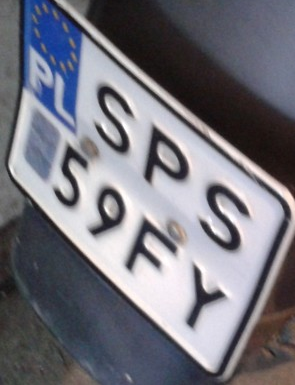
\includegraphics[width=\textwidth]{img/detect-bg-bad-input}
    \label{fig:detect_bg_bad_input}
    \caption{}
  \end{subfigure}
  ~
  \begin{subfigure}[b]{0.45\textwidth}
    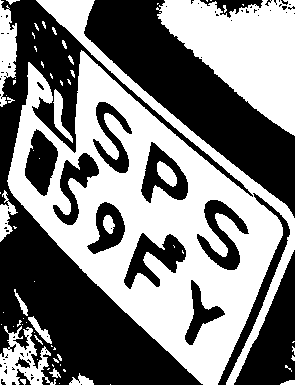
\includegraphics[width=\textwidth]{img/detect-bg-bad-output}
    \label{fig:detect_bg_bad_output}
    \caption{}
  \end{subfigure}
  \caption{Operacja progowania lokalnego}
  \label{fig:detect_bg_bad}
\end{figure}

\begin{figure}
  \centering
  
\includegraphics[width=7cm]{img/detect-bg-ok-output}
  \caption{Obraz po wykonaniu operacji usuwania znaków przez rozmycie medianowe}
  \label{fig:detect_bg_ok}
\end{figure}

\subsection{Różne kąty wykonania obrazu}
Bardzo często zdarza się, że obraz tablicy rejestracyjnej nie został wykonany idealnie na wprost obiektu. Efektem tego mogą być obrazy, których numery rejestracyjne są pochylone, co może powodować ich niepoprawną lokalizację oraz identyfikację. \\
\textbf{Algorytm detekcji kąta obrotu}. W tym szczególnym przypadku udało mi się rozwiązać ten problem w niżej opisany sposób. Wymaga on założenia, że tło tablicy rejestracyjnej jest jaśniejsze od pozostałych obiektów znajdujących się na obrazie, natomiast jeśli wcześniej zostanie zastosowany algorytm unifikacji tła tablicy rejestracyjnej, omawiany w poprzednim podrozdziale, warunek ten będzie spełniony.
\paragraph{}
Na początku, obraz poddajemy działaniu jednego z algorytmów progowania. Wynik tego progowania nie musi dawać nam bardzo dobrego rezultatu jeśli chodzi o rozdzielenie znaków od tła, ważne jest tylko, aby wyraźnie zostało zaznaczone tło. Można zastosować jeden z algorytmów progowania dynamicznego, lub progowania globalnego z wysokim progiem. Po zastosowaniu algorytmu progowania, znajdujemy największy spójny biały obszar, a następnie wyznaczamy najmniejszy prostokąt otaczający ten obszar. Kąt, pod jakim znajduje się prostokąt, jest kątem, o jaki obrócony został obraz podczas jego tworzenia.\\
Poszczególne kroki działania algorytmu zostały przedstawione na rysunku~\ref{fig:detect_image_angle}.

\begin{figure}
  \centering
  \begin{subfigure}[b]{0.45\textwidth}
    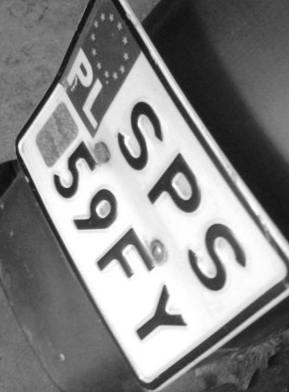
\includegraphics[width=\textwidth]{img/detect-image-angle-input}
    \label{fig:rzut_liczba_linii_jeden}
    \caption{}
  \end{subfigure}
  ~
  \begin{subfigure}[b]{0.45\textwidth}
    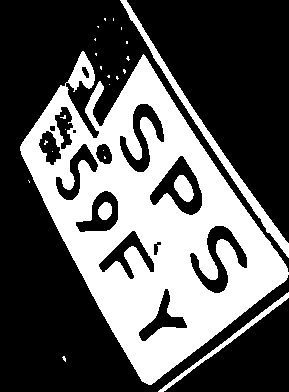
\includegraphics[width=\textwidth]{img/detect-image-angle-threshold}
    \label{fig:rzut_liczba_linii_dwa}
    \caption{}
  \end{subfigure}
  ~
  \begin{subfigure}[b]{0.45\textwidth}
    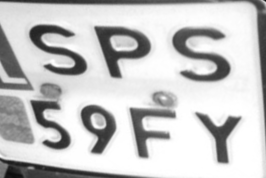
\includegraphics[width=\textwidth]{img/detect-image-angle-output}
    \label{fig:rzut_liczba_linii_dwa}
    \caption{}
  \end{subfigure}
  \caption{Wyniki operacji poszczególnych kroków algorytmu rotacji obrazu: a) obraz wejściowy, b) progowanie i znajdowanie prostokąta obejmującego, c) obraz wynikowy.}
  \label{fig:detect_image_angle}
\end{figure}


\subsection{Różne formaty zapisu danych}\label{ssec:different_formats}
Numer rejestracyjny pojazdu może być zapisany jako jedna, lub jako dwie linie tekstu. Założeniem algorytmu rozpoznawania tablic rejestracyjnych jest możliwość rozpoznania obydwóch formatów zapisu, dlatego przed przystąpieniem do dalszej analizy, należy określić liczbę linii tekstu. Znajomość liczby linii jest przydatna podczas oceny ostatecznego rozwiązania segmentacji obrazu, ponieważ znana jest wtedy przybliżona lokalizacja liter. Poniżej przedstawiam propozycję dwóch rozwiązań problemu detekcji liczby linii wykorzystanych do zapisu numeru rejestracyjnego.
\paragraph{Metoda rzutu jasności obrazu.} Algorytm rzutu jasności obrazu opisywany był na stronie~\pageref{ssec:rzut_jasnosci}. Zauważyłem, że algorytm ten może również zostać wykorzystany do określenia liczby linii tekstu, wykorzystując do tego tylko poziomy rzut jasności dla obrazu. Na rysunku~\ref{fig:rzut_liczba_linii} zamieszczone zostały dwa obrazy przedstawiające rzuty jasności dla tablicy rejestracyjnej zawierającej jedną, oraz dwie linie tekstu. Można zauważyć, że w miejscach, gdzie nie znajduje się tekst, wykres rzutu jasności osiąga wyraźne ekstremum. Dla jednej linii tekstu, wykres rzutu jasności powinien zawierać tylko dwa takie ekstrema (nad, oraz pod tekstem), natomiast dla tablicy zawierającej dwie line tekstu, wystąpić powinny trzy ekstrema (dodatkowe ekstremum znajdujące się pomiędzy dwoma wierszami tekstu).\\
Algorytm wyszukuje trzy największe maksimum lokalne na wykresie rzutu jasności, przy założeniu, że nie mogą znajdować się w odległości mniejszej niż $\frac{1}{3}$ wysokości obrazu (aby uniknąć znalezienia dwóch ekstremum należących do jednej białej linii). Na końcu sprawdzane były dwa warunki:
\begin{itemize}
  \item znalezione wartości maksymalne były porównywane z odchyleniem standardowym wyznaczonym z wartości rzutu jasności, i jeśli ich różnica od wartości średniej była większa niż wyznaczone odchylenie, warunek był spełniony,
  \item jeśli po posortowaniu ekstremum względem ich pozycji, druga wartość była wartością maksymalną spośród trzech znalezionych, warunek był uznany za spełniony.
\end{itemize}
W przypadku spełnienia przynajmniej jednego z powyższych warunków, na obrazie znaleziono dwie linie tekstu. W przypadku niespełnienia żadnego warunku, na obrazie znaleziono tylko jedną linię tekstu zawierającego numer rejestracyjny. Warto zauważyć, że algorytm nie zwróci poprawnych wyników w przypadku gdy obraz będzie obrócony. Aby wykluczyć takie przypadki, należy przed zastosowaniem metody rzutu jasności obrazu wykonać algorytm detekcji kąta i obrotu opisanego we wcześniejszym podrozdziale.


\begin{figure}
  \centering
  \begin{subfigure}[b]{0.45\textwidth}
    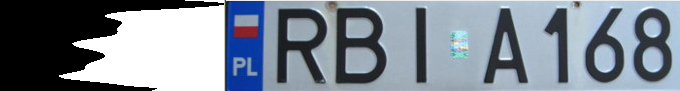
\includegraphics[width=\textwidth]{img/rzut-liczba-linii-jeden}
    \label{fig:rzut_liczba_linii_jeden}
    \caption{}
  \end{subfigure}
  ~
  \begin{subfigure}[b]{0.45\textwidth}
    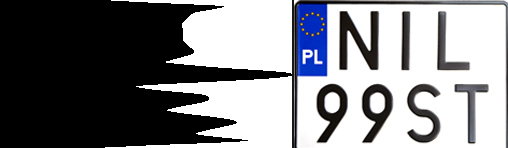
\includegraphics[width=\textwidth]{img/rzut-liczba-linii-dwa}
    \label{fig:rzut_liczba_linii_dwa}
    \caption{}
  \end{subfigure}
  \caption{Rzuty jasności dla tablic rejestracyjnych zawierających a) jedną linię b) dwie linie tekstu}
  \label{fig:rzut_liczba_linii}
\end{figure}

\paragraph{Metoda a priori: porównywanie lokalizacji.} Algorytm porównywania lokalizacji może zostać zastosowany, gdy znana jest lokalizacja wszystkich liter na obrazie oraz ich rozmiarów. Zauważyłem, że w przypadku numerów rejestracyjnych zapisanych w jednej linii, różnica odległości od górnej krawędzi poziomej obrazu nie różni się między każdym następnym znakiem o więcej niż 20\% średniej wysokości znaku. W metodzie ważne jest, aby porównywać ze sobą dwa kolejne znaki, ponieważ nie zakłada ona, że obraz nie został wykonany pod kątem.\\
Algorytm określania liczby linii metodą porównywania liczby lokalizacji przedstawiony został poniżej.
\begin{enumerate}
  \item Obliczyć średnią wysokość znaku.
  \item Umieścić wszystkie znaki w kolejce priorytetowej, gdzie priorytetem jest położenie znaku na osi poziomej obrazu.
  \item Pobrać znak z kolejki i zapisać do tymczasowej zmiennej.
  \item Pobrać znak z kolejki i dokonać porównania:
    \begin{gather*}
      abs(tmp.y - c.y) < 0.2*avg\_h,
    \end{gather*}
    gdzie $tmp$ to znak umieszczony w zmiennej tymczasowej, $c$ to znak pobrany z kolejki, a $avg\_h$ to średnia wysokość znaku. Wartość współczynnika $0.2$ została wyznaczona empirycznie - dla tej wartości otrzymywałem najlepsze wyniki podczas wykonywania testów. Jeśli warunek nie jest spełniony, numer rejestracyjny zapisany jest w dwóch liniach. Algorytm kończy działanie.
  \item Zapisać do zmiennej tymczasowej znak pobrany z kolejki.
  \item Jeśli kolejka nie jest pusta, przejść do punktu 4).
  \item Numer rejestracyjny został zapisany w jednej linii. Algorytm kończy działanie.
\end{enumerate}
Rysunek~\ref{fig:apriori_liczba_linii} przedstawia tablice rejestracyjne zawierające zapisane numery rejestracyjne zarówno w dwóch, jak i w jednej linii. Można zauważyć, że w przypadku tekstu zapisanego w jednej linii, pomimo pochylonego tekstu, algorytm powinien poradzić sobie z rozpoznaniem liczby linii, ponieważ każdy sąsiedni znak jest tylko nieznacznie przesunięty w górę względem znaku poprzedniego. W przypadku tekstu zapisanego w dwóch liniach, nawet jeśli tekst jest idealnie poziomo, algorytm rozpozna dwie linie tekstu, ponieważ maksymalna różnica pomiędzy początkami dwóch sąsiednich (pod względem odległości na linii poziomej) znaków na osi pionowej jest większa niż średnia wysokość znaku.

\begin{figure}
  \centering
  \begin{subfigure}[b]{0.45\textwidth}
    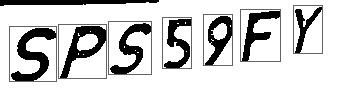
\includegraphics[width=\textwidth]{img/apriori-liczba-linii-jeden}
    \label{fig:apriori_liczba_linii_jeden}
    \caption{}
  \end{subfigure}
  ~
  \begin{subfigure}[b]{0.45\textwidth}
    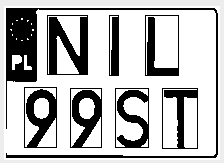
\includegraphics[width=\textwidth]{img/apriori-liczba-linii-dwa}
    \label{fig:apriori_liczba_linii_dwa}
    \caption{}
  \end{subfigure}
  \caption{Metoda rozpoznawania liczby linii tekstu dla obrazu: a) zawierającego jedną linię, b) zawierającego dwie linie tekstu.}
  \label{fig:apriori_liczba_linii}
\end{figure}

\subsection{Dodatkowe elementy na tablicach}\label{ssec:additional_elements}
Tablice rejestracyjne zawierają bardzo często elementy, które nie są elementami numerów rejestracyjnych, ale mogą zostać sklasyfikowane jako element numeru, podczas procesu segmentacji. Poniżej przedstawiam metody, jakie zastosowałem w celu filtracji elementów nieporządanych. Weryfikacji podlega każdy znaleziony segment, sprawdzane są wszystkie poniższe warunki.
\paragraph{Stosunek szerokości do wysokości znaku}\mbox{}\\
Zauważyłem, że w każdym znaku pojawiającym się w numerze rejestracyjnym, szerokość znaku jest mniejsza od jego wysokości. Warunek ten spełniony był dla każdej czcionki pojawiającej się w dostępnych danych, dlatego mogłem wykluczyć wszystkie segmenty, które nie spełniają warunku:
\begin{gather*}
  segment.H > segment.W,
\end{gather*}
gdzie W i H to odpowiednio szerokość i wysokość segmentu.

\paragraph{Minimalna wysokość znaku}\mbox{}\\
Podczas obserwacji danych testowych zauważyłem, że wysokość znaku numeru rejestracyjnego zapisanego na tablicy nie osiąga wartości mniejszej niż $\frac{1}{4}$ wysokości tablicy rejestracyjnej. Dlatego odrzucić można segmenty niespełniające warunku:
\begin{gather*}
  segment.H > \frac{I.H}{4},
\end{gather*}
gdzie segment.H to wysokość segmentu, a I.H to wysokość obrazu. Należy przyjąć, że wysokość obrazu pokrywa się z tablicą rejestracyjną.\\
Na rysunku~\ref{fig:min_height_condition} można zauważyć, że litery napisu ,,CALIFORNIA'' nie został oznaczone jako poprawne segmenty dzięki zastosowaniu warunku o minimalnej wysokości znaku. Gdyby warunek nie został zastosowany, prawdopodobnie mniejszy napis zostałby rozpoznany jako numer rejestracyjny pojazdu.

\begin{figure}
  \centering
  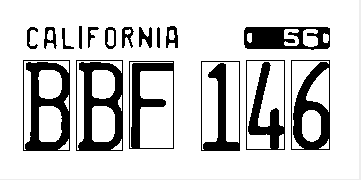
\includegraphics[width=10cm]{img/min-height-condition-output}
  \label{fig:detect_bg_bad_input}
  \caption{Obraz tablicy rejestracyjnej po procesie segmentacji}
  \label{fig:min_height_condition}
\end{figure}

\paragraph{Średnia wysokość znaku}\mbox{}\\
Numer rejestracyjny zawiera zwykle od sześciu do dziesięciu znaków, natomiast liczba dodatkowych elementów na tablicy rejestracyjnej zwykle nie jest większa niż dwa. Zauważyłem, że wyznaczając średnią wysokość segmentów, a następnie obliczając odchylenie standardowe, można odrzucić elementy, które nie spełniają warunku:
\begin{gather*}
  abs(E-segment.H) < \sigma,
\end{gather*}
gdzie:\\
$E$ - wartość średnia wysokości wszystkich znalezionych segmentów, \\
$segment.H$ - wysokość segmentu,\\
$\sigma$ - odchylenie standardowe w populacji wysokości segmentów.\\
Ten warunek pozwala na wyeliminowanie elementów, które kształtem przypominają znaki, natomiast ich wysokość wyróżnia się od innych znaków. Rysunek~\ref{fig:standard_deviation_condition} przedstawia dwa przykłady tablic rejestracyjnych, w których warunek ten uniemożliwił akceptację niepoprawnych elementów.
\begin{figure}
  \centering
  \begin{subfigure}[b]{0.65\textwidth}
    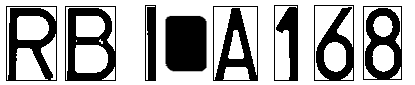
\includegraphics[width=\textwidth]{img/standard-deviation-condition-too-small}
    \label{fig:standard_deviation_too_small}
    \caption{}
  \end{subfigure}
  ~
  \begin{subfigure}[b]{0.40\textwidth}
    
\includegraphics[width=\textwidth]{img/standard-deviation-condition-too-big}
    \label{fig:standard_deviation_too_big}
    \caption{}
  \end{subfigure}
  \caption{Usuwanie fałszywych pozytywów poprzez porównanie ze średnią wysokością znaku: a) fałszywy pozytyw niższy niż znaki numerów rejestracyjnych, b) fałszywy pozytyw o większej wysokości niż przeciętny znak numeru rejestracyjnego}
  \label{fig:standard_deviation_condition}
\end{figure}
